% Options for packages loaded elsewhere
\PassOptionsToPackage{unicode}{hyperref}
\PassOptionsToPackage{hyphens}{url}
%
\documentclass[
]{article}
\usepackage{amsmath,amssymb}
\usepackage{iftex}
\ifPDFTeX
  \usepackage[T1]{fontenc}
  \usepackage[utf8]{inputenc}
  \usepackage{textcomp} % provide euro and other symbols
\else % if luatex or xetex
  \usepackage{unicode-math} % this also loads fontspec
  \defaultfontfeatures{Scale=MatchLowercase}
  \defaultfontfeatures[\rmfamily]{Ligatures=TeX,Scale=1}
\fi
\usepackage{lmodern}
\ifPDFTeX\else
  % xetex/luatex font selection
\fi
% Use upquote if available, for straight quotes in verbatim environments
\IfFileExists{upquote.sty}{\usepackage{upquote}}{}
\IfFileExists{microtype.sty}{% use microtype if available
  \usepackage[]{microtype}
  \UseMicrotypeSet[protrusion]{basicmath} % disable protrusion for tt fonts
}{}
\makeatletter
\@ifundefined{KOMAClassName}{% if non-KOMA class
  \IfFileExists{parskip.sty}{%
    \usepackage{parskip}
  }{% else
    \setlength{\parindent}{0pt}
    \setlength{\parskip}{6pt plus 2pt minus 1pt}}
}{% if KOMA class
  \KOMAoptions{parskip=half}}
\makeatother
\usepackage{xcolor}
\usepackage[margin=1in]{geometry}
\usepackage{graphicx}
\makeatletter
\def\maxwidth{\ifdim\Gin@nat@width>\linewidth\linewidth\else\Gin@nat@width\fi}
\def\maxheight{\ifdim\Gin@nat@height>\textheight\textheight\else\Gin@nat@height\fi}
\makeatother
% Scale images if necessary, so that they will not overflow the page
% margins by default, and it is still possible to overwrite the defaults
% using explicit options in \includegraphics[width, height, ...]{}
\setkeys{Gin}{width=\maxwidth,height=\maxheight,keepaspectratio}
% Set default figure placement to htbp
\makeatletter
\def\fps@figure{htbp}
\makeatother
\setlength{\emergencystretch}{3em} % prevent overfull lines
\providecommand{\tightlist}{%
  \setlength{\itemsep}{0pt}\setlength{\parskip}{0pt}}
\setcounter{secnumdepth}{-\maxdimen} % remove section numbering
\ifLuaTeX
  \usepackage{selnolig}  % disable illegal ligatures
\fi
\IfFileExists{bookmark.sty}{\usepackage{bookmark}}{\usepackage{hyperref}}
\IfFileExists{xurl.sty}{\usepackage{xurl}}{} % add URL line breaks if available
\urlstyle{same}
\hypersetup{
  pdftitle={09-18-24\_weekly-update},
  pdfauthor={Cappy Pugliese},
  hidelinks,
  pdfcreator={LaTeX via pandoc}}

\title{09-18-24\_weekly-update}
\author{Cappy Pugliese}
\date{2024-09-18}

\begin{document}
\maketitle

\hypertarget{last-week}{%
\subsubsection{Last Week}\label{last-week}}

\hypertarget{section}{%
\paragraph{9/9 - 9/13}\label{section}}

\begin{itemize}
\tightlist
\item
  finished reading most of the Forsythe 2021 paper
\item
  finished my individual development plan
\item
  practiced more with using github
\item
  learned about the cluster and started the sign up process
\item
  dropped one of my classes (conservation bio) since my courseload was
  too much
\end{itemize}

\hypertarget{this-week}{%
\subsubsection{This Week}\label{this-week}}

\hypertarget{section-1}{%
\paragraph{9/16 - 9/17}\label{section-1}}

\begin{itemize}
\tightlist
\item
  checked out \href{https://www.whitenosesyndrome.org/}{whitenose.org}
\item
  finished skimming through the rest of the Forsythe 2021 paper
\item
  skimmed through the other 2 WNS papers
\item
  tried to finish setting up cluster account

  \begin{itemize}
  \tightlist
  \item
    wasn't letting me reset my password for some reason
  \item
    but I might just have to wait a week or so
  \end{itemize}
\end{itemize}

\hypertarget{section-2}{%
\paragraph{9/18}\label{section-2}}

\begin{itemize}
\tightlist
\item
  downloaded fastQC to laptop
\item
  downloaded a random \emph{P. destructans} fastq file

  \begin{itemize}
  \tightlist
  \item
    had some trouble downloading the right file format, but then I
    figured it out
  \item
    tried to run it through fastQC
  \item
    there was a file format error
  \end{itemize}
\item
  decided it was a great time to start up my lab notebook

  \begin{itemize}
  \tightlist
  \item
    set up a repository in github
  \item
    figured out how to add r files to my repository
  \item
    figured out how to create r markdown files
  \item
    wrote this r markdown file
  \end{itemize}
\end{itemize}

\hypertarget{section-3}{%
\paragraph{9/19}\label{section-3}}

\begin{itemize}
\tightlist
\item
  tried to re-run the fastq file through fastQC

  \begin{itemize}
  \tightlist
  \item
    once again there was a file format error
  \item
    I tried downloading a different fastq file to see if it was just
    that particular file
  \item
    still recieved the same file format error
  \item
    downloaded it a different way again and still recieved the same file
    format error
  \item
    unsure of what I am doing wrong or if I need to go in and change the
    file format?
    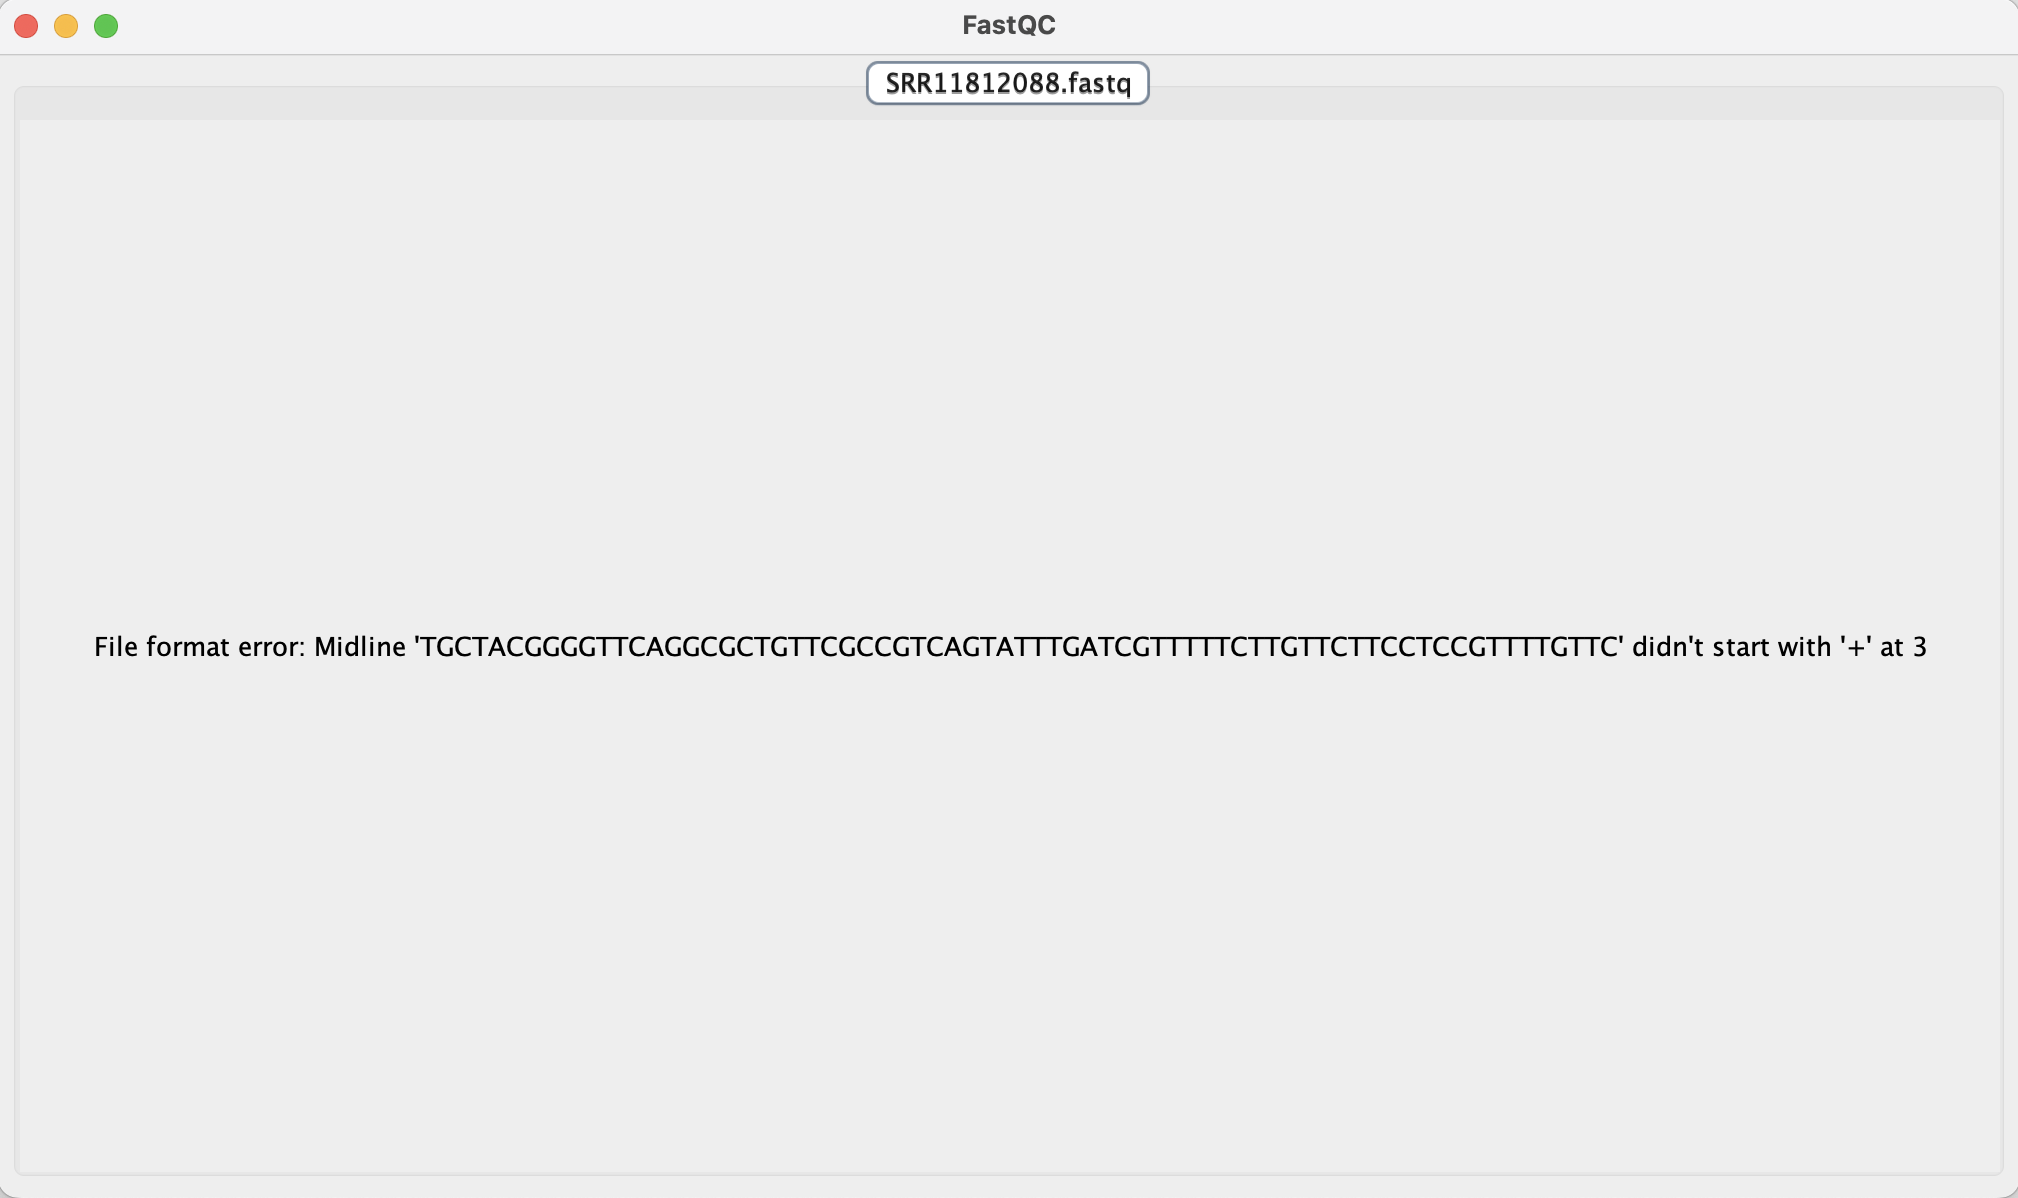
\includegraphics{images/fastq-file-error-message_09-19-24.png}
  \end{itemize}
\item
  watched some
  \href{https://github.com/CBC-UCONN/CBC_Docs/wiki/Intro-to-Xanadu-Videos}{xanadu
  intro videos}

  \begin{itemize}
  \tightlist
  \item
    learned how to use the terminal to sign into the head computer
  \item
    was able to successfully sign in and out of the cluster using the
    command line
  \end{itemize}
\end{itemize}

\end{document}
